\section[Hardware]{Hardware\footnote{Stephan and Abdul}}\label{Sec_Har}

\subsection[RFID reader and antenna]{RFID reader and antenna\footnote{Stephan}}
The RFID reader from KTS Systeme (see fig.\ref{Reader}) is a HF Modul (frequency around 13.56 MHz). It contains a full-fledged microcontroller with a high-performance RFID transceiver IC. It has a 1.27 mm pitch pin-headers for THT mounting. The connection to an external antenna can be realized via a Single ended 50$\Omega$ connection or via Pin Header U.FL. jack, which was used in this project. \\
\begin{figure}[!htbp]
\centering
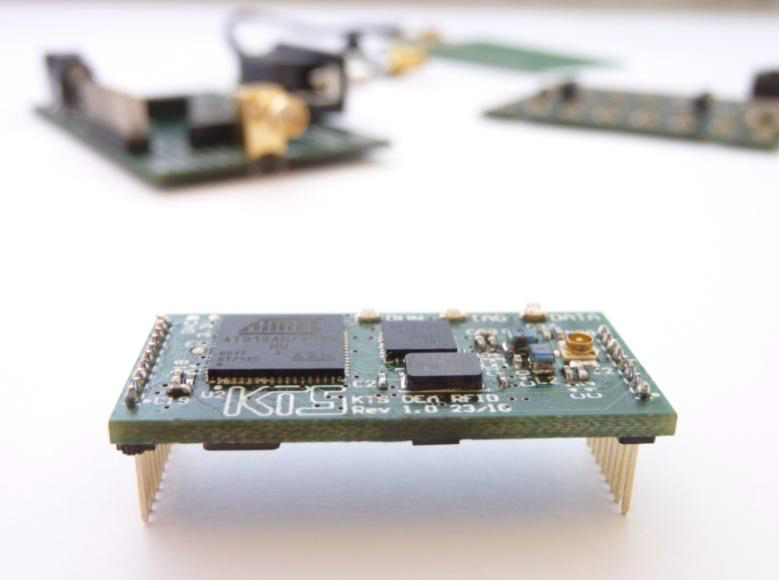
\includegraphics[width = 8cm]{Pictures/Reader}
\caption{RFID reader KTS Systeme RFIDM1356-001}
\label{Reader}
\end{figure}\\
The communication to other devices is realized via a UART compatible serial interface via pin 6 (RX) and 7 (TX). The power supply is a 5 V DC connection via pin 1 (VCC) and pin 10 (GND). The reader is standardized to ISO 15693 and ISO14443A/B and has the overall dimensions 36 x 16 x 4 mm [LxWxH]\cite{KTSSysteme.2017}.\\
The reader has three LEDs:\\
- Green: Run - Lights when reader receives power\\
- Yellow: Tag - Lights when a tag is detected\\
- Red: Data - Lights when data transfer to or from a tag\\
To configure the reader, KTS Systeme provides also a software (Tag2Image) for free. The reader was configured to scan the environment in an automatic anti collision mode (AT+Scan=AC,RSSI). Anti collision means that multiple tags can be detected at the same time and is highly important in this project. The output of the scan is a continuous information of the Identification (ID) and the Received Signal Strength Indicator (RSSI) of the detected tags. For example means: SCAN:+UID=E00402000018313E,+RSSI=7/6 that the tag with the ID (in hex) E00402000018313E was detected with a RSSI of 7/6. For the RSSI is the first number the value for the main and the second for the auxiliary receiver channel. In this project only the first number of the RSSI was used. The RSSI is an integer value from 0...7 and gives an information about the distance between the antenna and the detected tag. 0 stands for the maximum reading range which was mentioned to be around 15 cm. A detailed relation was figured out experimental during the project and will be explained later in this report. An AT Command Reference Guide is also available on http://rfid.kts-systeme.de/downloads/.\\
\\
The antenna (fig. \ref{Antenna}) is a HF PCB Antenne (PCBA1356$\_$8) also from the company KTS Systeme. It has a dimension of 80 x 80 mm. The connection to the reader is realized by a SMA jack and has a self-impedance of 50$\Omega$. The antenna is designed for passive tags in a frequency range around 13.56 MHz and has a maximum power of 1W. \\
\begin{figure}[!htbp]
\centering
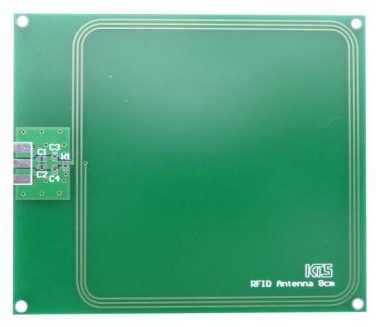
\includegraphics[width = 6cm]{Pictures/Antenna}
\caption{RFID Antenna KTS Systeme PCBA1356$\_$8}
\label{Antenna}
\end{figure}\\
The antenna and the reader are connected with a SMA to U.FL. adapter cable.\\

\subsection{RFID tag ?}

\subsection{Wifi modul (Abdul ?)}

\subsection{HW setup?!? (Abdul ?)}\label{Sec_Har_Set}